%\documentclass{article}
%
%\usepackage{tikz}
%\usetikzlibrary{arrows,shapes,chains,matrix,positioning,scopes,patterns,calc}
%\usepackage{color}
%
%\usepackage{latexsym}
%\usepackage{amsmath,amssymb,amsthm}
%\usepackage{etoolbox}
%
%\begin{document}

%Labels
%SystemModel %ChannelCoding %BEC 

\begin{tikzpicture}
\def \recW{1in}; %Encoder Length
\def \recH{0.5in}; %Encoder Width

\def \R{0.06in}; %Larger circle radius

\def \Gblks{0.25in}; %Gaps between blocks
\def \ext{0.95in}; %Extensions towards left and right of the figure
\def \extB{0.25in}; %Extensions towards top of the figure

\def \fsize{\Large}; %Defining a generic font size to be adjusted depending on the scaling

\tikzstyle{rect}   = [ rectangle, draw, text centered, thick,
                        minimum height=\recH, minimum width=\recW ]

\node [rect](enc) at (0,0) {\fsize{Encoder}} ;
\node (chan)  [right = \ext of enc,draw,rectangle,text centered,thick,minimum width=1.5in,minimum height=1.5in]    {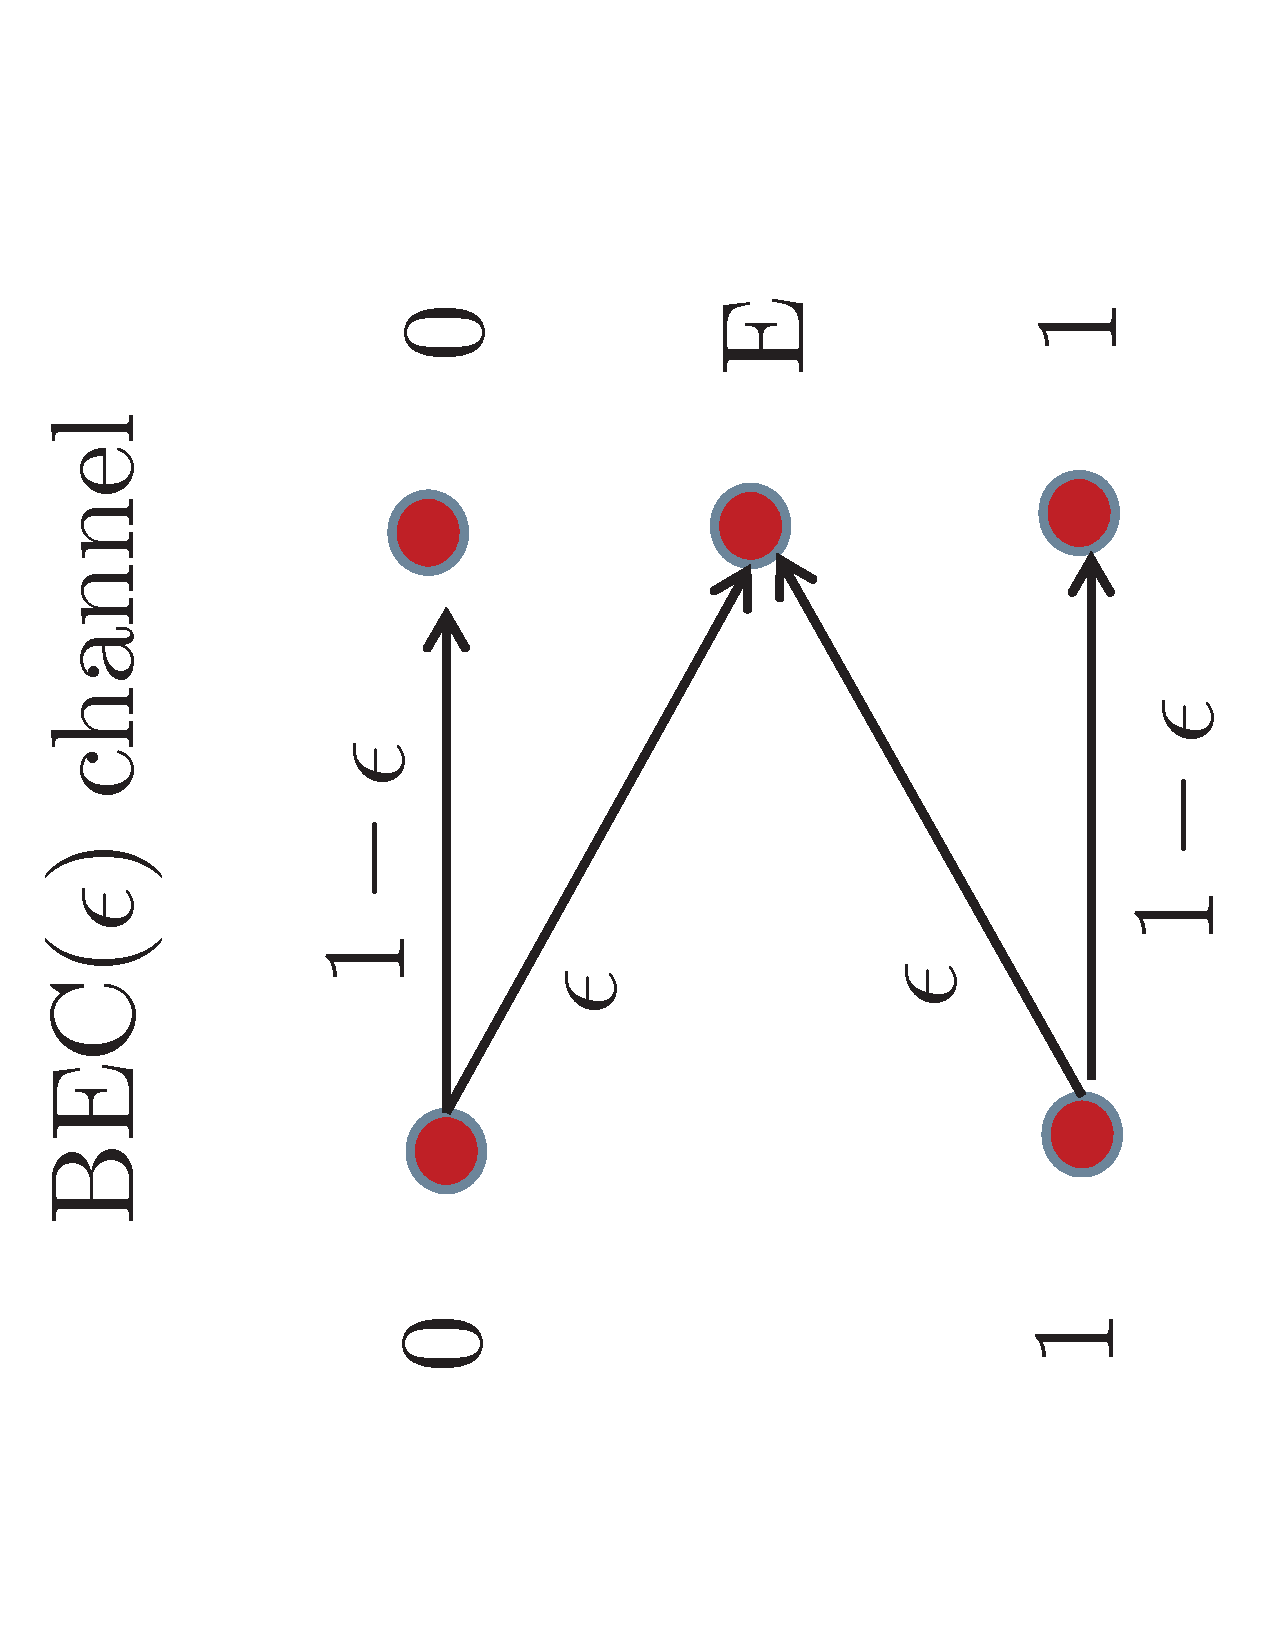
\includegraphics[width=1.5in,angle=-90]{BECchannelmodel.pdf}};
\node (dec)[rect,right=\ext of chan] {\fsize Decoder} ;

\draw[<-,thick](enc)-- +(-2*\ext,0) node[midway,above]{\fsize $m_1,\ldots,m_k$};
\draw[->,thick](enc)--(chan)node[midway,above]{\fsize $x_1,\ldots,x_n$}node[midway,below]{\fsize $x_i\in \{0,1\}$};
\draw[->,thick](chan)--(dec)node[midway,above]{\fsize $r_1,\ldots,r_n$}node[midway,below]{\fsize $r_i\in \{0,1\}$};;

%\draw[<-,thick](chan)--+(0,\extB) node[above] {\fsize $e_1,\ldots,e_n$};
\draw[->,thick](dec)--+(2*\ext,0)node[midway,above]{\fsize  $\hat{m_1},\ldots,\hat{m_k}$};

\end{tikzpicture}
%\end{document} 